\section{Historical Introduction}
Fractional calculus is a field which extends all the way back to the birth of \emph{ordinary} calculus. In this section we wish to give an account of the development of this field. Like any historical recount this section will have its flaws, inaccuracies and omissions. One can get bogged down in the historiography of the field and criticise this recount as a story written with whiggish bias, but we seek to tell a story which is relevant to the rest of this thesis an contextualize modern fractional calculus.

In any historical introduction to fractional calculus one almost always starts with the letters exchanged between L'Hopital and Leibniz in the fall of 1695. Upon hearing of Leibniz's calculus and the differential operator
\begin{align}
    \frac{d}{dx}
\end{align}
and it's generalisation
\begin{align}
    \frac{d^n}{dx^n}
\end{align}
L'Hopital asked Leibniz what it would mean to set $ n = \frac{1}{2} $. Leibniz responded saying that 
\begin{align}
    d^\frac{1}{2}x = x\sqrt{dx:x}
\end{align} and adding that
``It will lead to a paradox, from which one day useful consequences will be drawn'' (Or at least that what most modern translations say) \cite{Abbas2012}. The notation is unfamiliar to modern mathematics, but this comment actually doesn't really reveal anything about how one might go about computing
\begin{align}
    \frac{d^\frac{1}{2}f}{dx^\frac{1}{2}}.
\end{align}

\begin{wrapfigure}{r}{0.3\textwidth}
    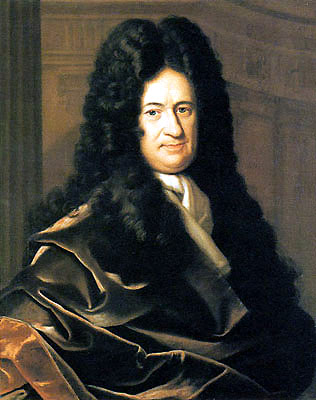
\includegraphics[scale=0.4]{images/Gottfried_Wilhelm_von_Leibniz}
    \caption{Bernhard Christoph Francke's portrait of Gottfried Wilhelm von Leibniz}
\end{wrapfigure}

Two years latter in letters to J. Wallis and J. Bernoulli Euler proposed a possible approach to dealing with fractional derivatives of exponential functions \cite{Abbas2012}. He noticed that
\begin{align}
    \label{eq:euler_frac}
    \frac{d^m}{dx^m} e^nx = n^me^{nx} 
\end{align}
and proposed that one could simply consider non-integer values of $ m $ in order to define a fraction differential operator. 
It is perhaps on this note that we should point out that the name \emph{fractional} calculus is a bit of a misnomer. As in the case above we do not require $ m \in \mathbb{Q} $, but rather are allowed to select $ m \in \mathbb{R} $ or even $ m \in \mathbb{C} $.

Given the definition / motivation in \eqref{eq:euler_frac} one might be tempted to use this result and extend it to other functions via the theory of Fourier Analysis. We need to keep in mind, however, that this was the late $ 17$th century and so Fourier had yet to be born, let alone develop the idea of Fourier decomposition and Fourier basis. This meant that at the time there was not \emph{obvious} way to extend this definition to other functions.

\begin{wrapfigure}{L}{0.25\textwidth}
    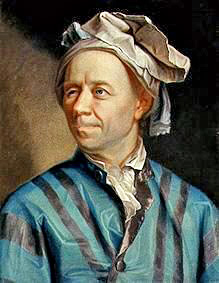
\includegraphics[scale=0.8]{images/Leonhard_Euler}
    \caption{1753 portrait of Leonhard Euler by Emanuel Handmann}
\end{wrapfigure}

Jumping forward a quarter of a century we arrive at the contributions of Euler. Euler made extremely important contributions in field of special functions, especially the Gamma function which turns out to be crucial in defining fractional integrals and fractional derivatives.

The Gamma function is essentially a solution to an interpolation problem, that is how to extend the factorial function to non-integer values of the argument. 



Although the problem of extending the factorial function had been considered by Daniel Bernoulli and Christian Goldbach in the 1720’s, it was eventually Euler who in a two letters, dated 13th October 1729 and 8th January 1730 respectively, gave two different representations of the factorial which could easily be extended to non-integer values. These were
\begin{align}
    \label{eq:euler_prod}
    n! = \prod_{k=1}^\infty \frac{\left(1+\frac{1}{k}\right)^n}{1 + \frac{n}{k}}
\end{align}
and
\begin{align}
    \label{eq:euler_log}
    n! = \int_0^1 (-\ln(s))^n ds.
\end{align}

Upon finding the first representation Euler could have simply stopped. He had found a formula which extended the factorial function to non-integer values. However he noticed that a special case of his product had already been calculated by Wallis. If we set $ n = \frac{1}{2} $ we get
\begin{align}
    \prod_{k=1}^\infty \frac{(1 + \frac{1}{k})^\frac{1}{2}}{1 + \frac{1}{2k}}
\end{align}
and squaring and multiplying by $ 2 $ we get
\begin{align}
    2 \left[ \prod_{k=1}^\infty \frac{(1 + \frac{1}{k})^\frac{1}{2}}{1 + \frac{1}{2k}}\right]^2 &= 2\prod_{k=1}^\infty \frac{1+\frac{1}{k}}{(1+\frac{1}{2k})^2} \\
    &= 2 \prod^\infty_{k=1} \frac{k^2+1}{(k + \frac{1}{2})^2} \\
    &= 2 \frac{2}{(1+\frac{1}{2})^2} \cdot \frac{5}{(2 + \frac{1}{2})^2} \cdot \frac{10}{(3+\frac{1}{2})^2}\cdots \\
    &= \frac{2}{1}\cdot\frac{2}{3}\cdot\frac{4}{3}\cdot\frac{4}{5}\cdots \\
    &= \prod_{k=1}^{\infty} \frac{4n^2}{4n^2-1}
\end{align}
and this last product had previously been calculated by Wallis and was known to be equal to $ \frac{\pi}{2} $. This meant that Euler had the result 
\begin{align}
    \frac{1}{2} ! = \frac{\sqrt{\pi}}{2}
\end{align}
We should point out that Wallis had calculated this result by considering 
\begin{align}
    \int_0^\pi \sin^n(x) dx
\end{align}
but this result is actually more easily obtained as a special case of Euler's infinite product for the sine function,
\begin{align}
    \sin(x) = x\prod_{k=1}^\infty \left( 1 - \frac{x^2}{k^2\pi^2} \right)
\end{align}
but Euler had not yet developed this.

The fact that Euler had $ \frac{1}{2} ! = \frac{\sqrt{\pi}}{2} $ piqued his curiosity and on nothing more than what appears to have been a hunch he went looking for an integral representation of $ n! $.
He arrived at \eqref{eq:euler_log} and it is here that our story returns to the history of fractional calculus. Aware of the fact that a meaning for $ \frac{d^\frac{1}{2}}{dx^\frac{1}{2}} $ was sought he noted that
\begin{align}
    \label{eq:euler_frac_deriv}
    \frac{d^m}{dx^m} x^n = \frac{n!}{(n-m)!}x^{n-m}
\end{align}
and then suggested that using either \eqref{eq:euler_prod} or \eqref{eq:euler_log} could give the necessary extension of meaning in order to define the derivative of the power function for non-integer orders of differentiation. In fact using Wallis' result along with a slight extension he was able to suggest that
\begin{align}
    \frac{d^\frac{1}{2}}{dx^\frac{1}{2}} x = \sqrt{\frac{4x}{\pi}}.
\end{align}
Although technically the modern notation we use for the Gamma function and the fact that $ \Gamma(n) = (n-1)! $ is due to Legendre, and were developed some considerable time after these ideas were first worked on by Euler, we will adopt the modern gamma function notation so as to make our discussions from this point more readable to those with some background knowledge. 

We would like to point out just how \emph{good} this idea for the definition of the fractional derivative by Euler was.
Firstly note that if we take $ n = 1 $ in \eqref{eq:euler_frac_deriv} we get that
\begin{align}
    \frac{d^{-1}}{dx^{-1}} x^m &= \frac{\Gamma(m+1)}{\Gamma(m+2)} x^{m+1} \\
    &= \frac{1}{m+1} x^{m+1} \\
    &= \int_0^x t^m dt
\end{align} 
which is consistent with the fundamental theorem of calculus. We discuss a modern version of this result in section \ref{sec:operators} of this thesis. 

Also in some formal sense this definition of the fractional derivative is consistent with that of Leibniz in that if we take a Taylor expansion of the exponential function we get that
\begin{align}
    e^{mx} = \sum_{k=0}^\infty \frac{m^k}{k!} x^k
\end{align}
and so without regard for convergence or any other technicalities one might be tempted to write
\begin{align}
    \label{eq:Euler_Leibniz_Sum}\
    \frac{d^r}{dx^r} e^{mx} &= \sum_{k = r}^\infty \frac{d^r}{dx^r} \frac{m^k}{k!} x^k \\
                            &= \sum_{k = r}^\infty \frac{m^k}{\Gamma(k+1)} \frac{\Gamma(k+1)}{\Gamma(k - r + 1)} x^{k-r} \\             
                            &= \sum_{k = r}^\infty \frac{m^k}{\Gamma(k - r + 1)}x^{k-r} \\
                            &= m^r \sum_{k = r}^\infty \frac{m^{k-r}}{\Gamma(k - r + 1)}x^{k-r}.
\end{align}
Letting $ j = k - r $ we have
\begin{align*}
    m^r \sum_{k = r}^\infty \frac{m^{k-r}}{\Gamma(k - r + 1)}x^{k-r}
        &= m^r \sum_{j = 0}^\infty \frac{m^{j}}{\Gamma(j + 1)}x^{j} \\
        &= m^r \sum_{j = 0}^\infty \frac{m^{j}}{j!}x^{j} \\
        &= m^r e^{mx}.
\end{align*}
and so in some formal sense these two definitions would at first glance appear to be consistent with each other.

This analysis has several problems. Firstly although the idea of expressing functions in terms of an infinite series dates back to perhaps the $ 14$th century the formal notion of a Taylor series dates back to $1715$ and Brook Taylor, only a few years before Euler's work in this field and it is not clear that such techniques would have been available to Euler. 

Secondly, and more importantly from a mathematical point of view, is the slight of hand played in \eqref{eq:Euler_Leibniz_Sum} where we essentially assume that if $ m > n $, $ \frac{d^m}{dx^m} x^n = 0 $. This is not the case if $ m \not\in \mathbb{Z} $. For example, using Euler's definition above we would have that
\begin{align}
    \frac{d^\frac{3}{2}}{dx^\frac{3}{2}} x = \frac{1}{\sqrt{\pi}} x^{-\frac{1}{2}} \neq 0.
\end{align}
One can see that in the integer case we get $ 0 $ simply because of singularities in the Gamma function for the non-positive integers. This particular complication of non-zero derivatives for the case where $ m > n $ extends even into more modern fractional derivatives and is dealt with in a modern context in section \ref{sec:operators} of this thesis.

It was almost a century latter when in 1822 Fourier suggest that using the equality
\begin{align}
    \label{eq:fourier_frac}
    \frac{d^m}{dx^m} f(x) = \frac{1}{2\pi} \int_{-\infty}^\infty \int_{-\infty}^\infty f(t)u^m \cos\left(ux - tu - \frac{m\pi}{2}\right) dt du
\end{align}
could give meaning to fractional derivative of a function. This appear to have been the first definition of a fractional derivative for a general class of \emph{sufficiently good} functions, in this case, for which \eqref{eq:fourier_frac} is defined.

\begin{wrapfigure}{R}{0.3\textwidth}
    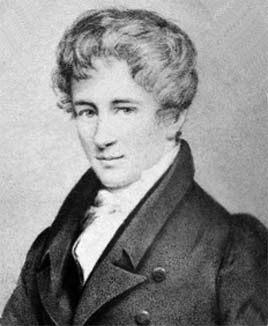
\includegraphics[scale=0.5]{images/Niels_Henrik_Abel}
    \caption{Johan Gørbitz's picture of Niels Henrik Abel.}
\end{wrapfigure}

The history of more modern fractional differential operators really begins with the Abel integral equation which was solved by Abel in papers dating back to 1823 and 1826. It was originally posed and solved in the context of the Tautochrone problem, which is finding the curve for which objects sliding under gravity without the effects of friction take equal times to reach their lowest point, independent of their starting point.

Abel's integral equation (of the first kind) is 
\begin{align}
    \label{eq:abel}
    \frac{1}{\Gamma(\alpha)} \int_0^x \frac{\phi(t)dt}{(x-t)^{1-\alpha}} = f(x) 
\end{align}
for $ x > 0 $ and $ 0 < \alpha < 1 $. Finding a \emph{solution} to this equation essentially means making $ \phi $ the subject. 
We demonstrate the solution method of this integral equation as it turns out to be important in latter formulations of fractional derivatives and integrals.
Firstly let's consider the integral 
\begin{equation}
	\label{eq:abel_int}
	I(x) := \int_a^x \frac{f(s)ds}{(x-s)^{1-\alpha}}.
\end{equation}
Now by substituting \eqref{eq:abel} into \eqref{eq:abel_int} we get 
\begin{align}
	I(x) &= \frac{1}{\Gamma(\alpha)} \int_a^x \frac{1}{(x-s)^{1-\alpha}} \left( \int_a^s \frac{\phi(t)dt}{(s-t)^\alpha} \right) ds \\
		&= \frac{1}{\Gamma(\alpha)} \int_a^x \left( \int_a^s \frac{\phi(t)dt}{(x-s)^{1-\alpha}(s-t)^\alpha} \right) ds
\end{align}
Now noting that the region of integration in $ \mathbb{R}^2 $ is just
\begin{align}
	a &\leq s \leq x \\
	a &\leq t \leq s 
\end{align}
which is equivalent to 
\begin{align}
	t &\leq s \leq x \\
	a &\leq t \leq x 
\end{align}
we can write 
\begin{align}
	\frac{1}{\Gamma(\alpha)} \int_a^x \left( \int_a^s \frac{\phi(t)dt}{(x-s)^{1-\alpha}(s-t)^\alpha} \right) ds 
		&= \frac{1}{\Gamma(\alpha)} \int_a^x \left( \int_t^x \frac{\phi(t)ds}{(x-s)^{1-\alpha}(s-t)^\alpha} \right) dt \nonumber \\
		\label{eqn:prebeta}
		&= \frac{1}{\Gamma(\alpha)} \int_a^x \phi(t) \left( \int_t^x (x-s)^{\alpha-1}(s-t)^{-\alpha} ds\right) dt. 
\end{align}
Now performing the substitution $ \tau = \frac{s-t}{x-t} $ yields 
\begin{align}
	\int_t^x (x-s)^{\alpha-1}(s-t)^{-\alpha} ds &= \int_0^1 \tau^{-\alpha} (1-\tau)^{\alpha - 1} d\tau \\
		&= B(1-\alpha,\alpha) \\
		&= \Gamma(1-\alpha)\Gamma(\alpha)
\end{align}
and so \eqref{eqn:prebeta} becomes
\begin{align}
	\frac{1}{\Gamma(\alpha)} \int_a^x \phi(t) \left( \int_t^x (x-s)^{\alpha-1}(s-t)^{-\alpha} ds\right) dt
		&= \frac{1}{\Gamma(\alpha)} \int_a^x \phi(t) \Gamma(\alpha)\Gamma(1-\alpha) dt \\
		&= \Gamma(1-\alpha)\int_a^x \phi(t) dt. 
\end{align}
So we have that 
\begin{align}
	\int_a^x \frac{f(s)ds}{(x-s)^{1-\alpha}} &= \Gamma(1-\alpha)\int_a^x \phi(t) dt
\end{align}
and by differentiating we get
\begin{align}
	\phi(x) &= \frac{1}{\Gamma(1-\alpha)} \frac{d}{dx} \int_a^x \frac{f(s)ds}{(x-s)^{1-\alpha}}
\end{align}
and so we have in some sense solved Abel's integral equation. Notice that we have not discussed which functions $ f $ are suitable. This is a bit of a tricky question and not really informative in the context of the rest of this thesis so we refer the interested reader to \cite{Samko1993}. 

As mentioned earlier Abel solved this integral equation in the context of the Tautochrone problem which corresponded to $ \alpha = \frac{1}{2} $. Abel seemingly had no actual desire to define a fractional integral or derivative but it turns out this problem can be recast in terms of fractional integral equation using a Riemann Liouville fractional integral and the result is in some sense a statement of a generalised fundamental theorem of calculus. We'll leave these ideas and turn our attention to the development of the Riemann-Liouville fractional integral and derivative and return to see how these ideas relate.

\begin{wrapfigure}{R}{0.3\textwidth}
    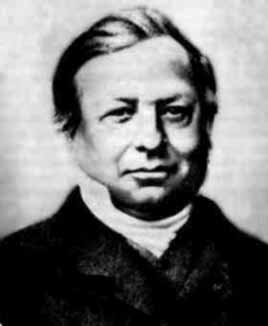
\includegraphics[scale=0.5]{images/Joseph_liouville}
    \caption{An updated and unattributed early photograph of Joseph Liouville.}
\end{wrapfigure}

It was in a collection of letters over six years from 1832 to 1837 that Liouville outlined ideas which hold any reasonable resemblance to modern fraction calculus. 

The first idea explored for a fractional derivative by Liouville bears someone of a resemblance to that of Fourier and Euler. 

If a function $ f $ can be expanded as 
\begin{align}
	f(x) = \sum_{k=0}^\infty c_k e^{a_kx}
\end{align}
then the fractional derivative of $ f $ of order $ \alpha $ could be written as
\begin{align}
	\frac{d^\alpha}{dx^\alpha} f(x) = \sum_{k=0}^\infty c_k a_k^\alpha e^{a_k x}
\end{align}
Note that by allowing complex values for $ a_k $ this is essentially a Fourier series and so the resemblance to Fourier's definition is apparent.

Despite the fact that we could view this series as a Fourier series, its not clear that this was done. Then the convergence of the series is tricky and it makes any consideration of the fractional derivative of $ f $ restrictive. 

In this series of letters he went on to derive a fractional integral
\begin{align}
	I^\alpha f(x) = \frac{1}{(-1)^\alpha \Gamma(\alpha)} \int_0^\infty f(x + t)t^{\alpha - 1} dt
\end{align}

Papers in 1832 and 1837 by Liouville were really the first papers which discussed an application of a fractional calculus, specifically to the solution of linear ordinary differential equations. 

He also discussed the idea of a fractional difference 
quotient.
Liouville didn't go far with this idea and it was considerably latter in 1867 and 1868 that Gr{\"u}nwald and respectively Letnikov dealt with this idea in much more depth. 
 
\begin{wrapfigure}{l}{0.3\textwidth}
    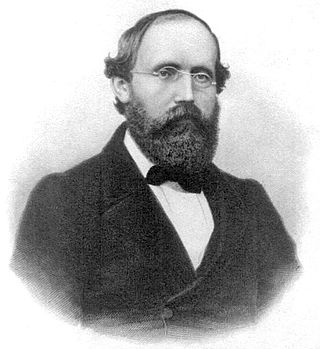
\includegraphics[scale=0.6]{images/Georg_Friedrich_Bernhard_Riemann}
    \caption{An 1863 image of Bernhard Riemann.}
\end{wrapfigure}

As a student in 1847 Riemann arrived at the fractional integral
\begin{align}
	I^\alpha f(x) = \frac{1}{\Gamma(\alpha)} \int_0^x \frac{f(t)dt}{(x-t)^{1-\alpha}}
\end{align}

Interestingly it wasn't until 10 years after his death in 1866 that this definition was published. Given the similarity of these fractional integrals these two ideas have been combined and named the Riemann Liouville fractional integral. This particular definition has become extremely significant and it forms the basis for modern fractional calculus. 

With a bit of technical fiddling it is quite easy to come up with a Riemann-Liouville fractional derivative. The idea behind this is discussed in section \ref{sec:operators}.

Although over the next hundred years or so there was significant development of other forms of fractional operators such the Gr{\u"}nwald Letnikov, Weyl, Miller Ross fractional derivatives. As we won't really explore these operators wi e will skip forward to Caputo in 1967. 

One of the problems with the Riemann-Liouville fractional derivative is that for many fractional differential equations the associated initial or boundary conditions must be of fractional order. Also the Riemann-Liouville fractional derivative of a constant is not zero. 

In two papers in 1967 and 1971 Michele Caputo\cite{Caputo1967} \cite{Caputo1971}, introduced a new fractional differential operator. These papers dealt with linear models of dissipation and interestingly this new operator resolved the issues to do with initial and boundary conditions along with the property that the Caputo fractional derivative of a constant is zero. It is perhaps interesting to note that this operator arose from purely physical considerations. 

\clearpage
